% !TeX root = main.tex
\chapter{平面几何}

\section{什么是共轭}

在抽象代数中我们接触过很多代数结构里的抽象概念,诸如正规化子,交换子,中心等等等等。
其中最先出现也最先困惑我们的就是\emph{共轭}这个概念。

\section{一个例子}
考虑Euclid平面的保距变换群(这个名词是什么并不重要)。\(g\) 表示是绕原点\(O\)
旋转\(\theta\degree\) 的旋转变换。\(h\) 表示沿向量\(v\) 的平移变换,
并把原点\(O\) 移动到点\(A\)。那么我们如何表示绕点\(A\) 旋转\(\theta\degree\)
的变换呢?很简单,先把\(A\) 点移动到\(O\) 点(对平面上的点做变换\(h^{-1}\)),
再做绕原点的旋转变换\(g\),最后再将原点平移至点\(A\) (做变换\(h\)),也就是做复合变换\(hgh^{-1}\)。
% TODO: Fix this
\begin{figure}[ht]
    \centering
    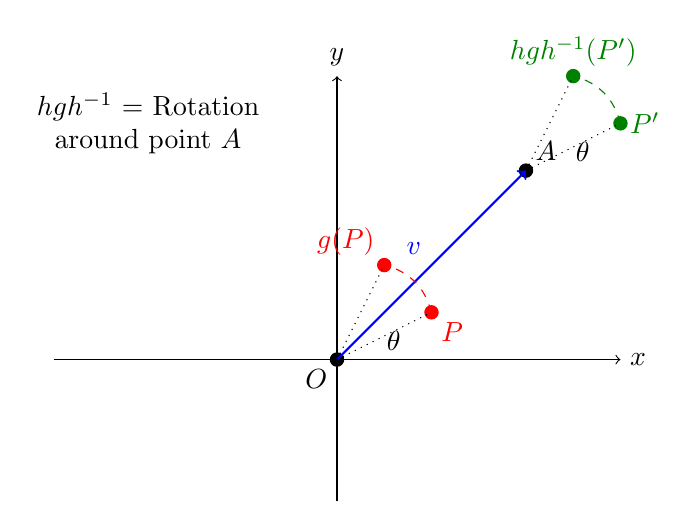
\begin{tikzpicture}[scale=1.2]
        % Coordinate system
        \draw[->] (-3,0) -- (3,0) node[right] {$x$};
        \draw[->] (0,-1.5) -- (0,3) node[above] {$y$};

        % Original point O and point A
        \filldraw[black] (0,0) circle (2pt) node[below left] {$O$};
        \filldraw[black] (2,2) circle (2pt) node[above right] {$A$};

        % Translation vector
        \draw[->, thick, blue] (0,0) -- (2,2) node[midway,
        above left] {$v$};

        % Point P and its image under rotation around O
        \filldraw[red] (1,0.5) circle (2pt) node[below right] {$P$};
        \filldraw[red] (0.5,1) circle (2pt) node[above
        left] {$g(P)$};
        \draw[->, dashed, red] (1,0.5) to[bend right] (0.5,1);
        \draw[dotted] (0,0) -- (1,0.5);
        \draw[dotted] (0,0) -- (0.5,1);
        \node at (0.6,0.2) {$\theta$};

        % Point P' = h(P) and its image under rotation around A
        \filldraw[green!50!black] (3,2.5) circle (2pt)
        node[right] {$P'$};
        \filldraw[green!50!black] (2.5,3) circle (2pt)
        node[above] {$hgh^{-1}(P')$};
        \draw[->, dashed, green!50!black] (3,2.5) to[bend
        right] (2.5,3);
        \draw[dotted] (2,2) -- (3,2.5);
        \draw[dotted] (2,2) -- (2.5,3);
        \node at (2.6,2.2) {$\theta$};

        % Explanation labels for conjugation
        \node[align=center] at (-2,2.5) {$hgh^{-1}$ =
        Rotation\\around point $A$};
    \end{tikzpicture}
    \caption{共轭变换 $hgh^{-1}$ 表示绕点 $A$ 旋转 $\theta$ 度}
\end{figure}

瞧,这正是共轭的定义。

\section{什么是共轭}

\begin{quotation}
    One way to think about conjugation is as a
    generalization of changing coordinates when rewriting
    matrices or, from a physical point of view, as the
    process of "seeing a group from a different perspective."

    In other words, what conjugation does in terms of group
    actions (and it is always a good idea to think of groups in
    terms of their actions) is it corresponds to a "change of
    coordinates" on the underlying set \(X\)
    . This is a basic reason conjugation and group theory are
    important in understanding Newtonian mechanics (where \(G\)
    is the Galilean group) or relativity (where \(G\)
    is the Lorentz group) or really much of modern physics in
    general: in physics groups are always studied because of
    their actions and we always want our concepts and equations
    to be invariant under these actions. (For example, mass and
        charge are invariant concepts. The mass or charge of an
    object doesn't change when you rotate or translate it.)

    This gives a very intuitive definition of a normal
    subgroup: it's a subgroup that "looks the same from every
    perspective." For example, the subgroup of translations in
    the Euclidean group is always normal because the
    description "\(g\)
    is a translation" is the same from every perspective (that
    is, it's invariant under conjugation). It's a good exercise
    to look at some groups you're familiar with and see if you
    can identify which subgroups are normal based on this
    principle. (This principle underlies the importance of
    normal subgroups in Galois theory as well.)
\end{quotation}

从我个人的理解来看,共轭起``重命名''的作用,具有换基的功能。
它可以把原先作用在原点处的东西转化为在别处的作用,从而让别的地方``旋转''成为了可能。

\section{为什么共轭如此神奇}
读完以上内容不免心生疑惑,为什么共轭如此神奇?为什么一个简单的\(hgh^{-1}\) 组合就能实现换基?
就以刚刚的例子为例,为什么平移变换复合过后旋转中心就变到了\(A\) 点?难道在复合的过程中旋转不会变形吗?

这个问题其实可以拆成两个部分:
\subsection{为什么在复合的过程中旋转不会变形?}
什么是变形?

事实上,我们考虑全体以原点为中心的旋转构成的子群。我们不难发现把旋转转换到\(A\) 点的\(hgh^{-1}\)
已经并不属于这个子群。在这个意义上,这个变换已经变形了。

如果``不变形''指的是变换过后的旋转依然是一个旋转,实际上平面上全体旋转构成的集合压根不构成一个群。

\subsection{为什么 \(hgh^{-1}\) 组合能实现换基?}

\href{https://math.stackexchange.com/questions/11971/intuition-behind-conjugation-in-group-theory}{讨论}
